\documentclass{article}
\usepackage[utf8]{inputenc}
\usepackage{amsmath}
\usepackage{listings}
\usepackage{geometry}
\usepackage{graphicx}
\usepackage{subfig}
\usepackage{cancel}
\usepackage{gensymb}
\usepackage[colorlinks=true]{hyperref}
\title{%
A real bounce in your step\\
\large Obligatory Assignment 2 \\
FYS 2160 at the University of Oslo}
\author{Simen Løken}
\date{October 2020}
\footskip = 90pt
\topmargin = -40pt

\begin{document}
\nocite{sourc7}
\nocite{sourc1}
\maketitle
\section{Abstract}
In this article we'll show and weigh different solutions to storing potential energy in a shoe. We'll also calculate these, and discuss how certain real results don't correspond with their theoretical results.
\section{Introduction}
Ever since the dawn of time, man's main method of transportation has been to use his feet. And although we no longer solely rely on our feet to travel, other activities have ensured that our feet haven't become entirely obsolete. I am of course referring to sport, more precisely, I'll be talking about running, and even more precisely, the energy conversation you can attain using polymers and the right kind of shoes. \newline
In mankind's never-ending quest to optimize just about everything, not even your shoes are safe. Nike's Vapourfly model of shoe boasts about a whopping 87\% energy return when rebounding off of the ground. Now that's a pretty good deal if you ask me, and they're doing it by using their new ZoomX foam material, a kind of polymer, which we'll be discussing here.
\section{Theory and Method}
Energy storage and the idea of storing energy in compressed objects isn't exactly a new concept. Springs, for example metal ones, also store energy. \newline You might recall, that the force on a spring can be expressed as:
\begin{equation*}
    F = kx
\end{equation*}
\newline where $F$ is the force exerted on the spring to deform it by a length of $x$. $k$ is the characteristic factor and a constant of the rigidity of the spring. This is Hookes law, andf rom this we can integrate this relation to find:
\begin{equation}
    PE = \int F \,dx = \int kx \,dx = \frac{1}{2} k x^2
\end{equation}
\newline Of course, the corresponding kinetic energy in such a system would be:
\begin{equation}
    KE = \frac{1}{2} mv^2
\end{equation}
where $m$ is the mass of the object connected to the spring, and $v$ is it's velocity. \newline
If we then assume a downwards motion, like for a shoe with springs hitting the ground, we'd get the relation:
\begin{equation} \label{1}
    KE_1 + \cancel{PE_1} = \cancel{KE_2} + PE_2 - LE_2 = KE_3 + \cancel{PE_3} - LE_2
\end{equation}
where 1 is on impact with the ground, 2 is at max compression of the spring, and 3 is when the spring is back in equilibrium. LE is an unknown variable representing the energy lost to lower forms of energy, like heat or sound. It's worth mentioning that there is probably and $LE_1$ and $LE_3$ also, but, in my opinion, the chief contributor to energy loss happens when compressing the spring, and as such I'm assuming $LE_1$ and $LE_3$ are minimal or close to zero.
\newline
Obviously, we'd ideally like for $LE_2$ to be as small as possible.
\newline
However, there's another option. Like previously discussed in the introduction, we can alternatively use polymers as a method of retaining the energy we have on impact. The closest thing we can relate this to would be a rubber band. Now the interesting thing about rubber bands, or rather polymers, is that they experience a decrease in entropy when stretched. This is the driving force behind the idea of using polymers for cushioning and storing energy in running shoes. \newline
You see, as opposed to a regular spring, when compressing (stretching) a polymer all the work is immediately thermal energy, same as for an ideal gas compressed in a piston. We can derive this from:
\begin{equation*}
    \Delta G = \Delta H - T \Delta S
\end{equation*}
where G is free energy, H the enthalpy and S is the entropy. T is temperature. Since the act of stretching, or compressing, is not spontaneous, $T\Delta S$ must be negative. Remind yourself that T is given in Kelvin, which is only ever positive, as such, $\Delta S$ must be negative, which means that when we stop compressing the polymers, the resulting reaction will be spontaneous, given us a negative $\Delta G$, and consequently a positive $\Delta H$ and $\Delta S$ 
\newline Such a system is driven entirely by entropy changes at a given temperature, and because the free energy derives entirely from the entropy change, the work done is entirely from thermal energy in the polymer, with a 100\% efficiency of conversion of thermal energy to work. Do note that this is also the case for ideal gases.\newpage
\section{Results}
According to the NYTimes \cite{sourc5}, whilst jogging we take an average of 140 steps per minute. That means we step $\frac{7}{3}$ times a second. Knowing this, we can approximate the acceleration (and velocity) of our feet coming down and touching the ground. This means that an average step takes about 0.45s. Let's assume we spend about 0.25s on the ground+raising our foot, meaning our time in the air is 0.2s. Know also that according to The Guardian \cite{sourc6}, the average weight of an Olympic runner is 69.2kg
\begin{equation*}
    v = v_0 + at = 0 + -9.81 m/s^2 \cdot 0.2s = -1.962 m/s
\end{equation*}
Knowing this, we can approximate our kinetic energy as we hit the ground to be:
\begin{equation*}
    KE_1 = \frac{1}{2}mv^2 = \frac{1}{2} 69.2kg \cdot -1.962^2 m/s = 133 J
\end{equation*}
This means that $LE_2 = \frac{1}{2} KE$, assuming 50\% loss from \cite{sourc4}, and:
\begin{equation*}
    KE_3 = 66.6 J
\end{equation*}
\newline
Now, I can't provide any calculations in regards to the efficiency of a polymer solution to energy retention, but we can probably deduce the reasoning as to why we get a 86\% return on energy as opposed to the 100\% theoretical return. I'm guessing this is excess energy getting lost as sound energy. We know that, unlike springs, all thermal energy is being converted 100\% back to kinetic energy when we stop compressing and stretching the polymers. There will also likely be some thermal energy lost as a result of friction against the surface we're running on.
\section{Discussion}
While we weren't able to precisely calculate the conservation of energy in polymer-soled shoes, we atleast managed to deduce a possible reasoning as to why it deviates from the theoretical 100\% return when converting kinetic energy to thermal in a polymer.
\newline
I'm also not so sure what kind of calculations or plots you'd like for me to do. I debated having a plot where I looked at the optimal $k$ given a weight $m$ when the sole is $l$ tall, but decided against it as it wasn't very relevant to the question. \newline
I'd also like to point out that I felt the values when calculating $KE_3$ were a bit large, seeing as 66.6 J means an upwards velocity of 1.39. That being said, it probably does not matter as it was only to illustrate in practice.
\section{Conclusion}
We've shown and discussed the different properties of a spring-loaded shoe vs a polymer-loaded(?) shoe. We've additionally looked at it's theoretical outputs, and weighed them against reality as a way to explain why we got the results we got. We've also shown in practice what a 50\% return on energy would look like.
\bibliographystyle{unsrt}
\bibliography{citations.bib}
\newpage
\section*{Appendices}
\subsection*{Appendix A - Calculations: all answers to part one of the assignment}
\begin{itemize}
    \item a) \textbf{If you study a single cycle, what is the change in the
entropy of the gas?}
\newline It is specified that the cycle is reversible, and as such, the entropy must be unchanged after one whole cycle.
    \item b) \textbf{Calculate $\Delta S_{23}$ and $\Delta S_{41}$ and show that this leads to $T_3^\gamma T_1 = T_2^\gamma T_4$.} 
    \newline Knowing what we know from a), we can deduce that the entropy in $\Delta S_{23}$ and $\Delta S_{41}$ must be equal but opposite. Therefore, we can calculate:
    \begin{equation*}
        \Delta S_{23} = \Delta S_{41}
    \end{equation*}
    \begin{equation*}
        C_p \ln{\frac{T_3}{T_2}} = -C_v \ln{\frac{T_4}{T_1}}
    \end{equation*}
    \newline
    We can then get rid of the natural logarithms, and we find using logarithm rules that:
    \begin{equation*}
        T_3^\gamma T_1 = T_2^\gamma T_4
    \end{equation*}
    \item c) \textbf{Show that $T_1 V_1^{\gamma -1} = T_2 V_2^{\gamma -1}$ and $T_3 V_3^{\gamma -1} = T_4 V_1^{\gamma -1}$.}
    \newline Using the first law of adiabatic compression, we can find that:
    \begin{equation*}
        \frac{T_2}{T_1} = \left(\frac{V_1}{V_2} \right)^{\gamma -1}
    \end{equation*}
    which can easily be rewritten as:
    \begin{equation*}
        T_1 V_1^{\gamma -1} = T_2 V_2^{\gamma -1}
    \end{equation*}
    The same is true for the other equation, as it is the same process, just the other way.
    \begin{equation*}
        \frac{T_3}{T_4} = \left(\frac{V_1}{V_3} \right)^{\gamma -1}
    \end{equation*}
    \begin{equation*}
        T_3 V_3^{\gamma -1} = T_4 V_1^{\gamma -1}
    \end{equation*}
    \item d) \textbf{Find $Q_{41}$ and $Q_{23}$.}
    \newline 
    \begin{equation*}
        Q_{23} = \Delta h = C_p \Delta T = C_p(T_3 - T_2)
    \end{equation*}
    \begin{equation*}
        Q_{41} = -\Delta U = - C_V (T_4-T_1)
    \end{equation*}
    Note that there is no work being done in this process, and W is therefore 0 and crossed out.\newline
    We find $Q_{41}$ in much the same way:
    \begin{equation*}
        Q_{41} - \cancel{W} = \Delta U = C_V \Delta T = C_V(T_1 - T_4)
    \end{equation*}
   \item e) \textbf{Find the ideal efficiency as function of the adiabatic constant $\gamma$, the compression ratio $r_k = V_1/V_2$ and the expansion ratio $r_l = V_1/V_3$.}
   \newline
   The ideal efficiency of a diesel engine is:
   \begin{equation} \label{ap1}
       \eta = 1 - r_k^{1-\gamma} \left( \frac{r_l^\gamma -1}{\gamma (r_l -1) }\right)
   \end{equation}
   \newline This is not yet relevant, but do note that for the Otto Cycle, $r_k = r_l$. 
   \item f) \textbf{Find some reasonable values of the volume and pressure of an engine and calculate the heat and work done in each step. Verify your answer in the previous exercise by calculating the efficiency of the
motor you have envisioned.}
   \newline
   First, we'll need to define some initial variables here. For simplicities sake, let's assume that we're operating at $T_1 = 300K$ (room temperature). $C_V, C_p$ and $\gamma$ are all known at this temperature, and are given as: $C_V = 0.718 \frac{kJ}{kg K}, C_p = 1.005 \frac{kJ}{kg K}$ and $\gamma = 1.4$ \cite{sourc2}. Let's also assume a standard ammount of pressure, $P_1 = 100 kPa$. We also need to assume by what factor the volume changes, let's assume it increases by a factor of 6 between $1\xrightarrow{} 2$ and a factor 2 between $2\xrightarrow{} 3$.
   \newline
   Knowing this, we can start:
   $$T_2 = T_1\left(\frac{V_1}{V_2}\right)^{\gamma-1}$$
   $$T_2 = 300K \cdot 6^{0.4} = 614K$$
   $$P_2 = P_1 \left(\frac{V_1 T_2}{V_2 T_1}\right)$$
   $$P_2 = 100 kPa \left( 6\frac{614}{300} \right) = 1228 kPa$$
   $$T_3 = T_2 \frac{V_3}{V_2}$$
   $$T_3 = 614K \cdot 2 = 1228K$$
   $$P_3 = P_2 $$
   $$P_3 = 1228 kPa$$
   $$Q_{23} = \Delta h = C_p (T_3 - T_2)$$
   $$Q_{23} = 1.005(1228-614)K = 617$$
   $$T_4 = T_3 \left( \frac{V_3}{V_4}\right)^{\gamma-1}$$
   $$T_4 = 1228K \left( \frac{2}{6} \right)^{0.4} = 791 K$$
   $$P_4 = P_3 \frac{V_3 T_4}{V_4 T_3}$$
   $$P_4 = 1228 kPa \frac{2\cdot 791 K}{8\cdot 1228 K} = 263 kPa$$
    $$Q_{41} = C_V(T_4-T_1)$$
    $$Q_{41} = 0.718(791-300)K = 353 kJ/kg $$
    \newpage
    For clarities sake, let's sort this into a table:
    \begin{table}[ht!]
        \centering
        \begin{tabular}{c|c|c}
             &T [K]& P [kPa]  \\
            1& 300& 100 \\
            2& 614& 1228 \\
            3& 1228&  1228 \\
            4& 791& 263&
        \end{tabular}
        \caption{All temperatures and pressures}
        \label{tab:1}
    \end{table}
    \newline and
    \begin{table}[ht!]
        \centering
        \begin{tabular}{c|c}
             &Q [kJ/kg]  \\
            2 $\xrightarrow{}$ 3& 617 \\
            4 $\xrightarrow{}$ 1& 353& 
        \end{tabular}
        \caption{Heat in and out}
        \label{tab:2}
    \end{table}
\newline
Using this, we can find our efficiency with the formula:
\begin{equation*}
    \eta = \frac{W_{net}}{Q_{in}} = \frac{617 kJ/kg - 353 kJ/kg}{617 kJ/kg} = 43\%
\end{equation*}
    \item g) \textbf{How could you in practice produce the highest possible efficiency?
} \newline No. You would not be able to produce the maximum possible efficiency, which in this case would be the Carnot efficiency. In an absolutely ideal scenario, that's to say, not possible in the real world, according to \cite{sourc3}: \newline \textit{"The ideal Otto cycle achieves the Carnot efficiency of an engine working between the maximum, pre-combustion, temperature and the intake temperature. This means that the ideal Otto cycle cannot achieve the Carnot efficiency determined by the highest and lowest temperature during the cycle."} \newline It is worth mentioning that this is regarding the standard Otto Cycle, not the Diesel Cycle with which we're working with here. \newline
Out of curiosity I decided to try and plot efficiency as a function of temperature, in addition to varying volume factors, shown on the next page below:
\begin{figure}[ht!] \label{fig1}
\centering
\subfloat[General Equation]{
  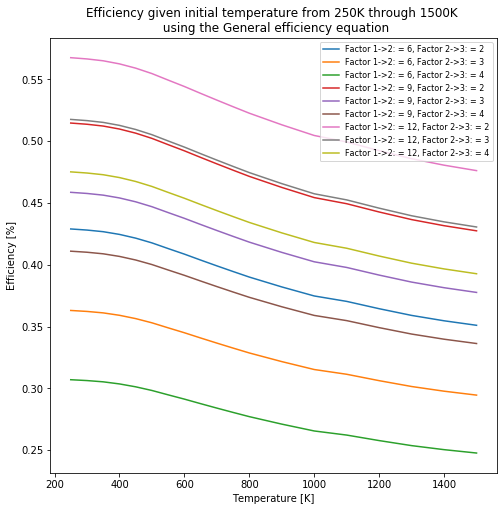
\includegraphics[width=75mm]{figure1.png}
}
\subfloat[Diesel Equation]{
  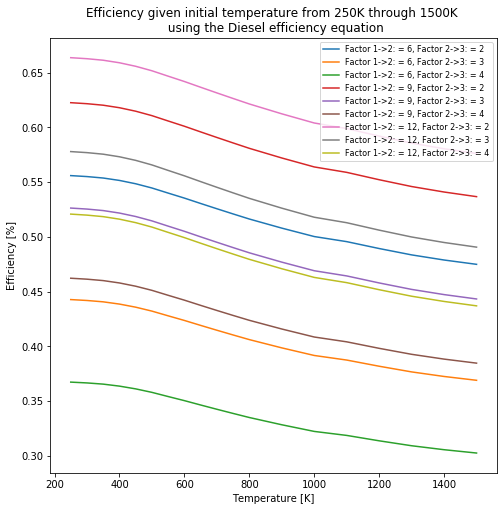
\includegraphics[width=75mm]{figure2.png}
}
\caption{Two different plots showing the efficiency given a temperature and varying volume factors. \newline
Factor 1 is the change in volume from $1\xrightarrow{} 2$ while Factor 2 is the change in volume from $2 \xrightarrow{} 3$. \newline I retrieved the values for $C_V, C_p$ and $\gamma$ from \cite{sourc2}.}

\end{figure}
\newpage
It is worth mentioning however that there are likely some issues with this model, as I'm having trouble believing that a diesel engine would be more efficient at -27\degree C versus 23\degree C. What we are seeing that I could believe however, is that bigger discrepancies in volume between 1 and 2, or rather, $\Delta V$ for $1\xrightarrow{} 2$. What this means essentially, is that as we compress and apply more force onto our fuel, we'll experience an increase in efficiency accordingly. This is however, probably pointless in reality, as the extra force we'd need to apply to get any noticeable increase in effect would likely far exceed whatever extra mileage we'd get.
\end{itemize}
\clearpage
\subsection*{Appendix B: Python Code for plots in 1g)}
\begin{lstlisting}[language=Python]
import numpy as np
import matplotlib.pyplot as plt

Cp = np.array([1.003,1.005,1.008,1.013,1.020,1.029,1.040,1.051,1.063,1.075,
               1.087,1.099,1.121,1.142,1.155,1.173,1.190,1.204,1.216])
Cv = np.array([0.716,0.718,0.721,0.726,0.733,0.742,0.753,0.764,0.776,0.788,
               0.8,0.812,0.834,0.855,0.868,0.886,0.903,0.917,0.929])
vol1 = [6,9,12]; vol2 = []
for k in vol1:
    vol2.append(k/3)
T = np.array([250,300,350,400,450,500,550,600,650,700,750,800,900,
              1000,1100,1200,1300,1400,1500])
def eff(T1, vol1, vol2, Cv,Cp):
    g = Cp/Cv
    T2 = T1*vol1**(g-1)
    T3 = T2*vol2
    T4 = T3*(vol2/vol1)**(g-1)
    Q1 = Cp*(T3-T2)
    Q2 = Cv*(T4-T1)
    netW = Q1-Q2
    eff = netW/Q1
    return eff
def eff2(T1, vol1, vol2, Cv,Cp):
    g = Cp/Cv
    eff = 1- 1/vol1**(g-1) * ((vol2)**g - 1)/(g*(vol2)-1)
    return eff
p = str(input("General Efficiency or Diesel Efficiency? [G/D] \n"))
p = p.lower()
if p == 'g':
    mode = eff; s = 'General'
elif p == 'd':
    mode = eff2; s = 'Diesel'
else:
    raise ValueError('Not recognized input. Please enter G or D only')
plt.figure(figsize=(8,8))
for i in range(len(vol1)):
    for j in range(len(vol2)):
        plt.plot(T, mode(T,vol1[i],vol2[j],Cv,Cp),
                 label='Factor 1->2: = %i, Factor 2->3: = %i' %(vol1[i],vol2[j]))
plt.title("""Efficiency given initial temperature from 250K through 1500K 
          using the %s efficiency equation""" %(s))
plt.xlabel('Temperature [K]'); plt.ylabel('Efficiency [%]')
plt.legend(fontsize=8)
plt.show()
\end{lstlisting}
\end{document}
